
\section{SIVIA Algorithm}

\vspace{0.3 cm}
	
	\textcolor{blue} {David DUVERGER}
	
	\vspace{0.5 cm}
	
	We will present here the fusion of the paving of the Gascogne Golf, the robots and their erosion. So, it is the resolution of the following mathematical formula:
	
	$$X(t) = G \cap F_{\delta}(X(t-\delta)) \cap g^{-1}([di,\infty])$$
	

\begin{algorithm}
  \caption{SIVIA algorythm}
  \vspace{0.5 cm}
  \textbf{Inputs}% Inputs section
  \begin{algorithmic}[1]
    \STATE Area $X0$
    \STATE Object $France$
    \STATE Object $Erosion$
    \STATE Object $Robots$
    \STATE Float $Precision$
  \end{algorithmic}
  \bigskip

  \textbf{Output}% Output section
  \begin{algorithmic}[1]

    \STATE Boxes $France U Robots U Erosion$
    \STATE Boxes $Robots U Erosion$
    \STATE Boxes $Sea$
  \end{algorithmic}
  \bigskip
  
  \textbf{Initialization}% Initialization section
  \begin{algorithmic}[1]
   	\STATE $stack\gets X0$
	\STATE $BoxesFranceURobotsUErosion\gets []$
	\STATE $BoxesRobotsUErosion\gets []$
	\STATE $BoxesSea\gets []$
  \end{algorithmic}
  
\end{algorithm}




\newpage


\begin{algorithm}
  \caption{SIVIA algorythm (continued)}
  \begin{algorithmic}
	\WHILE{len of stack >0}
	
		\vspace{0.3 cm}
	
  		\STATE $X\gets Interval \hspace{0.1cm} Vector \hspace{0.1cm} of \hspace{0.1cm} stack$
		\STATE $FranceTest\gets France.function(X)$
		\STATE $ErosionTest\gets Erosion.function(X)$ 
		\STATE $RobotsTest\gets Robots.function(X)$

		\vspace{0.3 cm}

  	 	\textcolor{blue}{//If we are in the France, robots or erosion:}\
	 	
	 	\IF{FranceTest==IBOOL.IN or ErosionTest == IBOOL.IN or RobotsTest == IBOOL.IN}
     	  	\STATE $Add \hspace{0.1cm} X \hspace{0.1cm} to \hspace{0.1cm} BoxesFranceURobotsUErosion$
     	
	 	\vspace{0.3 cm}
	 	
	 	\textcolor{blue}{//If we are in the robots or erosion:}\
	 	 \IF{RobotsTest == IBOOL.IN or ErosionTest == IBOOL.IN}
     		\STATE $Add \hspace{0.1cm} X \hspace{0.1cm} to \hspace{0.1cm} BoxesRobotsUErosion$
	 	 
	
	 	 \ENDIF
	 	 
	 	 \vspace{0.3 cm}
     		
     	\textcolor{blue}{//Else if we are outside all:}\
	 	 \ELSIF{ $FranceTest == IBOOL.OUT \hspace{0.1cm} and \hspace{0.1cm}  ErosionTest == IBOOL.OUT \hspace{0.1cm} and \hspace{0.1cm}  RobotsTest == IBOOL.OUT$}
	 	 \STATE $Add \hspace{0.1cm} X \hspace{0.1cm} to \hspace{0.1cm} BoxesSea$
	 	 
     	\ELSE
     
      	\vspace{0.3 cm}
     			\IF{Size \hspace{0.25cm} of \hspace{0.1cm} X > Precision}
          			\STATE $(X1, X2)\gets cut \hspace{0.3cm}  X$
          			\STATE $Add \hspace{0.3cm}  X1 \hspace{0.3cm}  in \hspace{0.3cm}  stack$
         			\STATE $Add \hspace{0.3cm}  X2 \hspace{0.3cm}  in \hspace{0.3cm}  stack$
         		\ENDIF
         	
  		\ENDIF
  		 \vspace{0.3 cm}
 	 \ENDWHILE 
	
	\vspace{0.3 cm}
	
  return BoxesFranceURobotsUErosion,BoxesRobotsUErosion,BoxesSea


  \end{algorithmic}
\end{algorithm}


\clearpage



\newpage

	With the help of this algorythm we can have a paving of the intersection between the Gascogne Golf, the robots and their erosion. We arrive to obtain the following result:
	

	
	\begin{figure}[!h] 
    \center
    	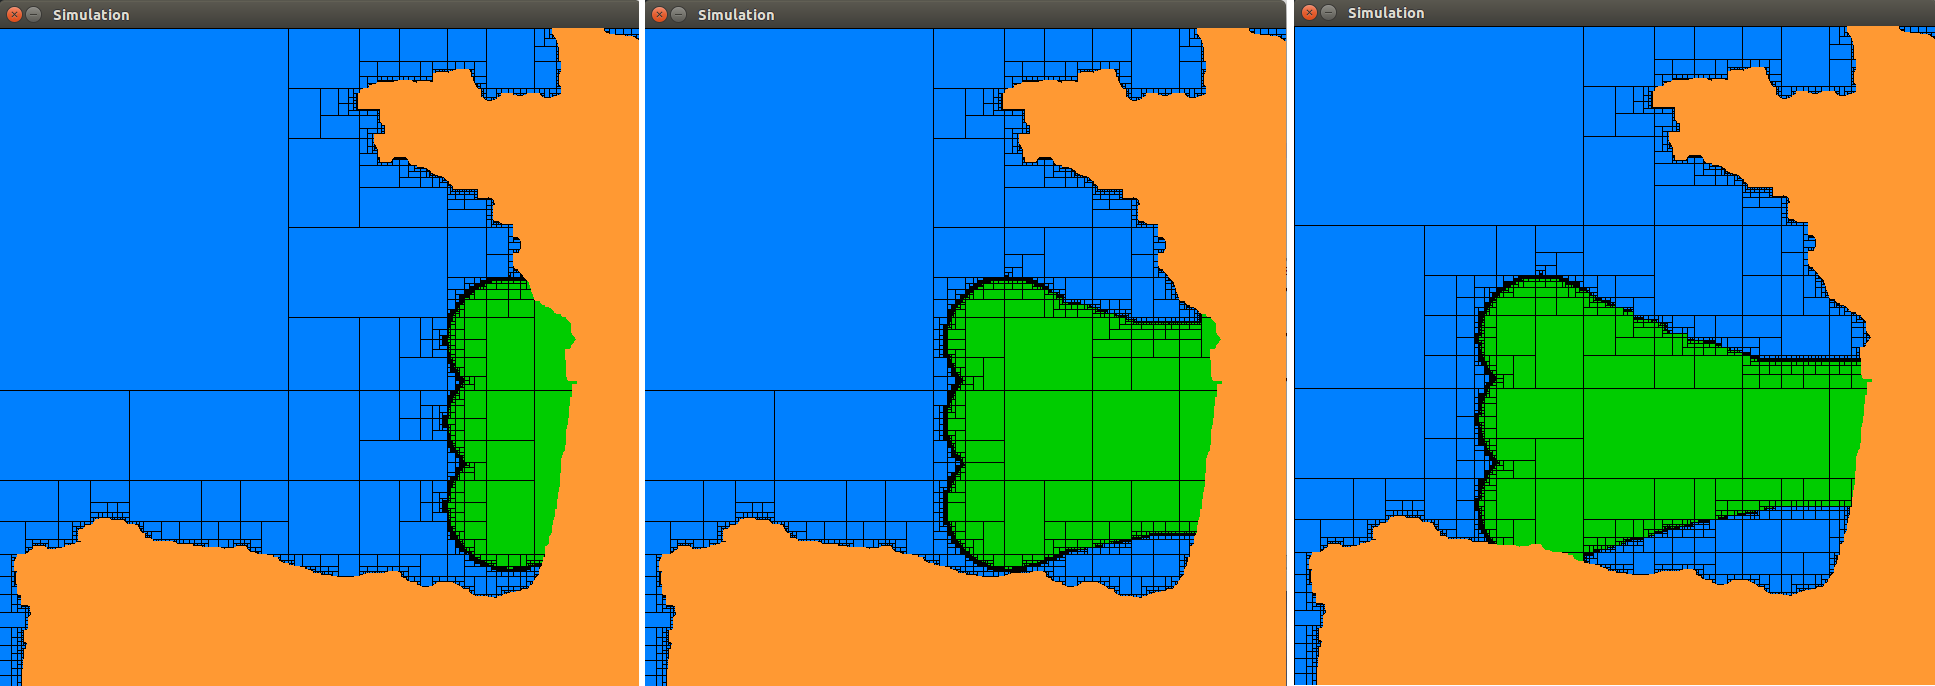
\includegraphics[scale=0.3]{SimulationFusion.png} 
    	\caption{Paving of the intersection between the Gascogne Golf, the robots and their erosion } 
    \label{S1 U S2}
	\end{figure} 
